% Modultest fugt og temp print

%tekst

I følgende afsnit testes temperatur- og fugtighedssensoren samt lavpasfilteret monteret på printet sammen med. Der testes for om temperatur og fugtighedsændringer registreres korrekt og om omregningen fra DC-niveau til værdi stemmer overens med scenariet i test. Scopbillederne er taget med et agilent oscilloskop.

Første test laves ved stuetemperatur. Til test af SHT21P sensoren bruges et færdigt termometer og fugtighedsmåler, af modellen [MODEL PÅ BJØRNS TERMOMETER], På billedet ses det at begge sensorer er i samme rum og at de bliver udsat for samme forhold. 

\begin{figure}[h]
\centering
{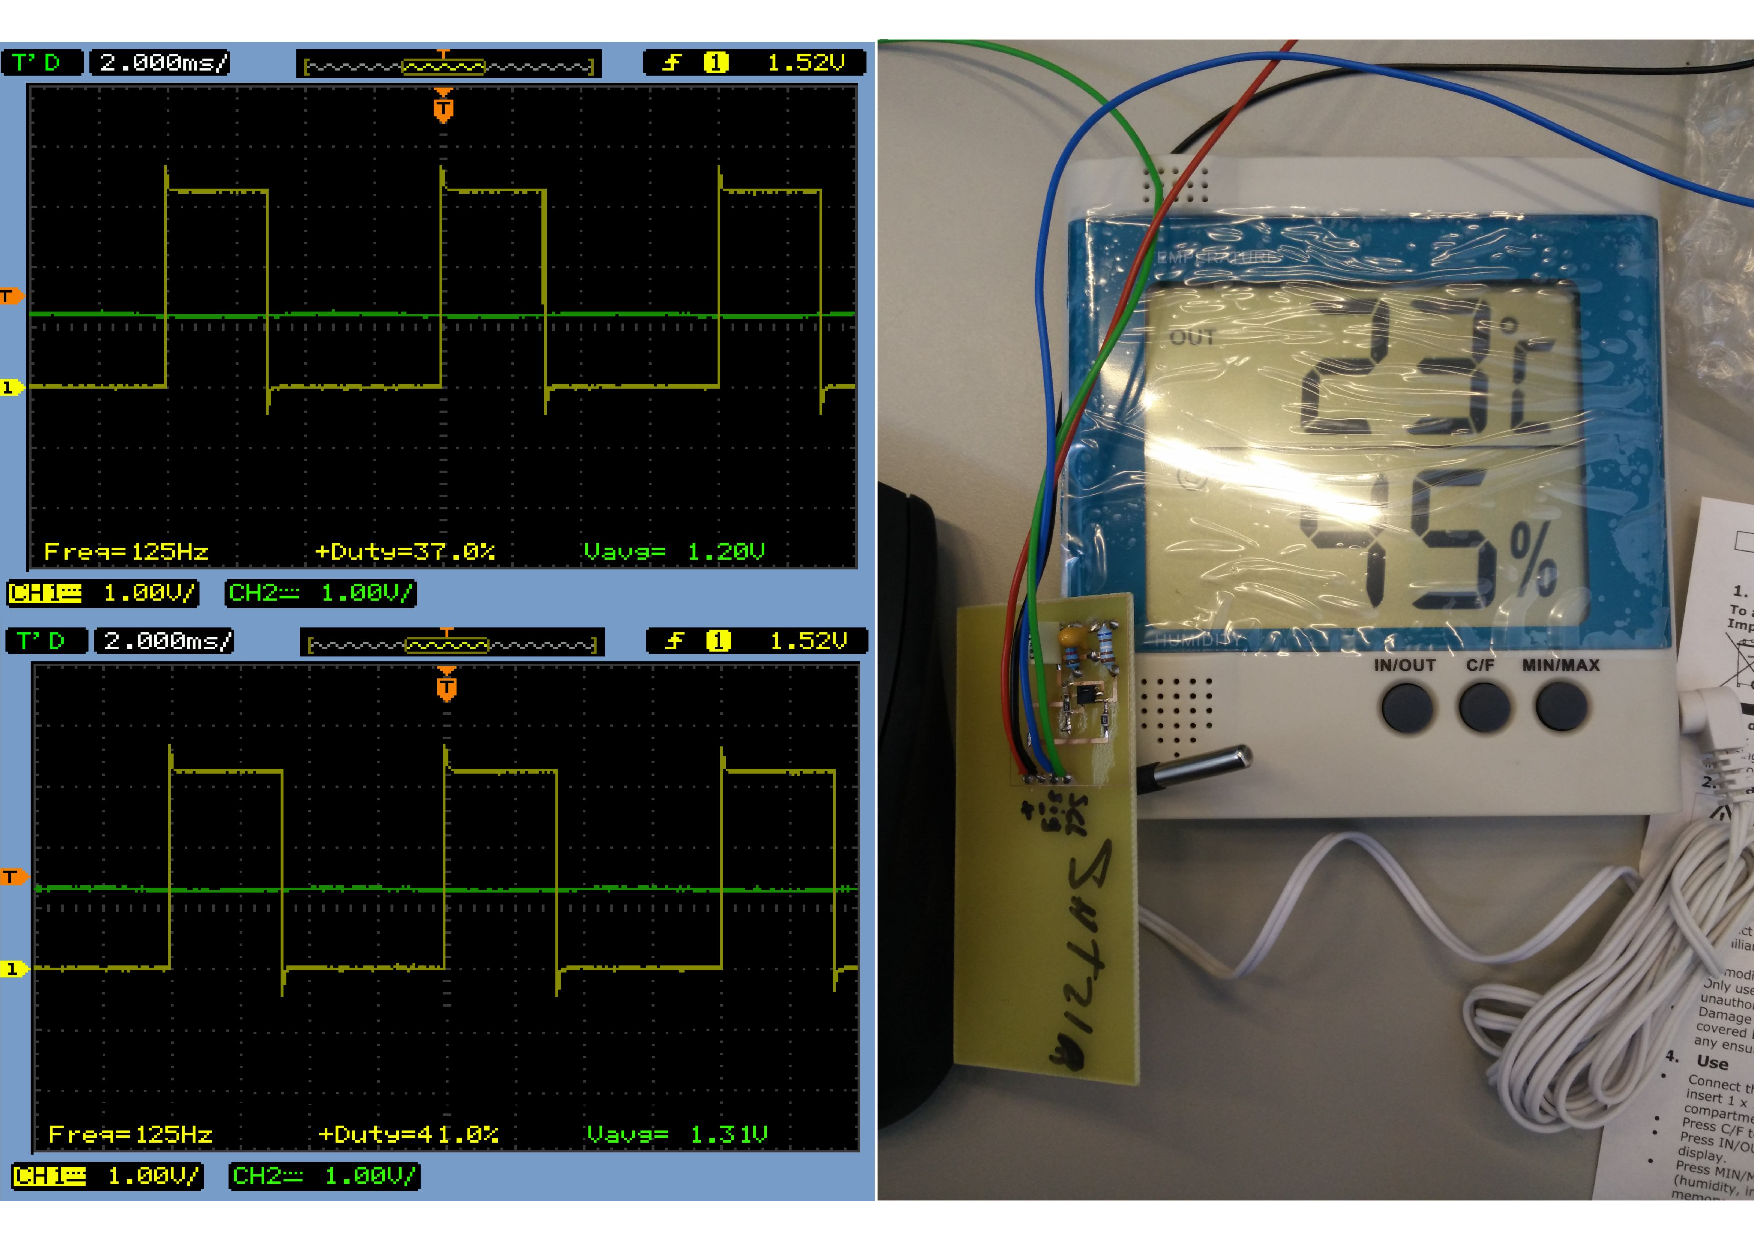
\includegraphics[width=0.90\textwidth]{filer/modultest/Billeder/test_stue}}
\caption{Billede af test incl. oscilloskop billede}
\label{lab:test_stue}
\end{figure}

Som scop billedet viser måles både en DC og et PWM signal. DCen er signalet efter lavpasfilteret og PWMen er den rå data fra sensoren. 
Sensorens SCL-ben er sat højt og sensoren måler derfor fugtighed. PWMen måles til at have en dutycycle på XX \% og spændingen efter filteret måles til XX V. Ud fra databladet kan dutycyclen omregnes til fugtighed med følgende formel:

[LIGNING FOR FUGTIGHED MED PWM]

Med følende formel regnes fugtigheden ud fra DC-værdien.

[LIGNING FOR FUGTIGHED MED DC]

SCL-benet ligges nu lav og temperaturen måles.Ud fra PWM regnes nu temperaturen.

[LIGNING FOR TEMPERATUR MED PWM]

Temperaturen regnes ud fra DCen som følger. 

[LIGNING FOR TEMPERATUR MED DC]


For at teste andre forhold bruges en varmepistol til at hæve temperatur og sænke fugtigheden. 
Samme målinger foretages:

\begin{figure}[h]
\centering
{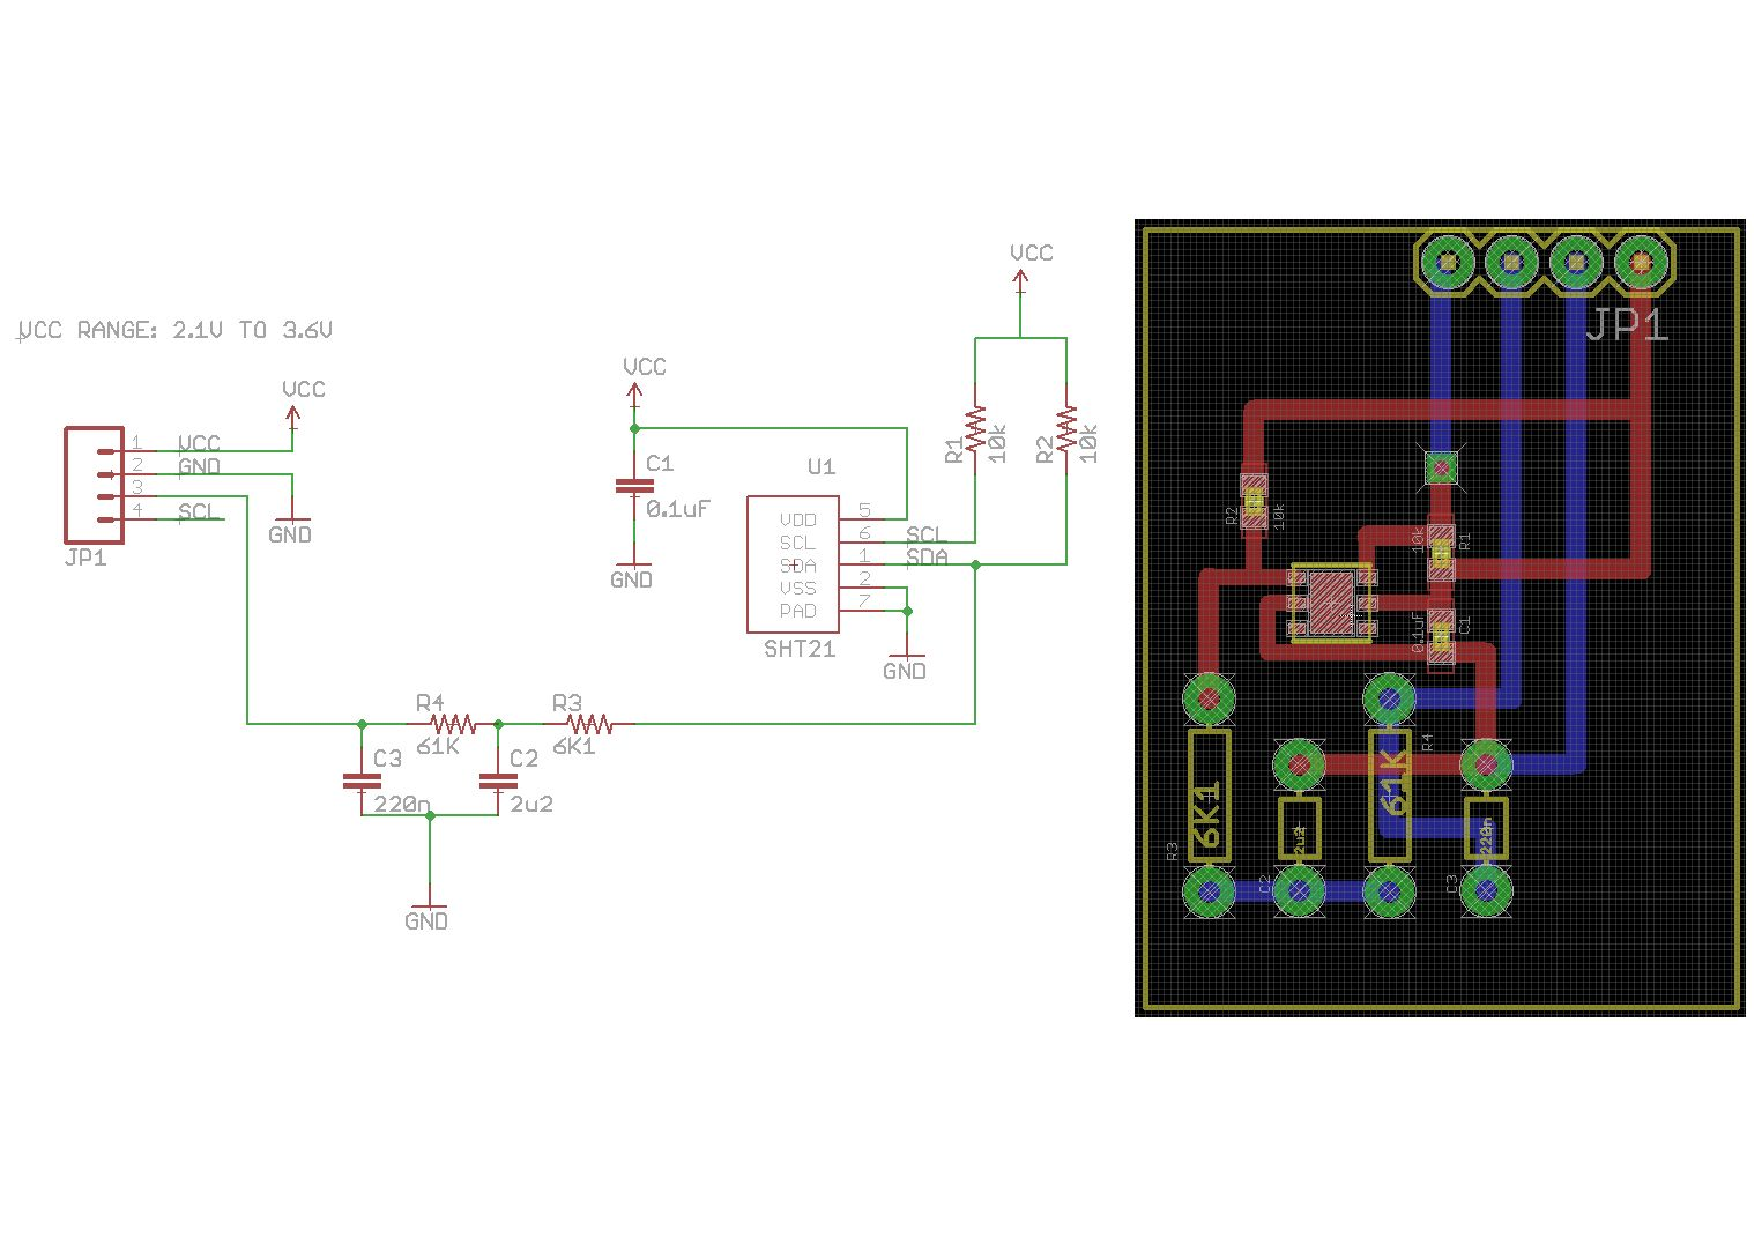
\includegraphics[width=0.90\textwidth]{filer/modultest/Billeder/test_varmt}}
\caption{Billede af test incl. oscilloskop billede}
\label{lab:test_varmt}
\end{figure}

Igen regnes værdierne for temperatur og fugtighed ud fra PWMen med en dutycycle på XX \% og DCen med en amplitude på XX V


[LIGNING FOR FUGTIGHED MED PWM]

Med følende formel regnes fugtigheden ud fra DC-værdien.

[LIGNING FOR FUGTIGHED MED DC]

SCL-benet ligges nu lav og temperaturen måles.Ud fra PWM regnes nu temperaturen.

[LIGNING FOR TEMPERATUR MED PWM]

Temperaturen regnes ud fra DCen som følger. 

[LIGNING FOR TEMPERATUR MED DC]

